% Use only LaTeX2e, calling the article.cls class and 12-point type.

\documentclass[12pt]{article}

% Users of the {thebibliography} environment or BibTeX should use the
% scicite.sty package, downloadable from *Science* at
% www.sciencemag.org/about/authors/prep/TeX_help/ .
% This package should properly format in-text
% reference calls and reference-list numbers.

\usepackage{scicite}
\usepackage[]{algorithm2e}
\usepackage{amsmath,amssymb}
\usepackage{amsthm}
\usepackage{bbm}
\usepackage[utf8]{inputenc}
\usepackage[english]{babel}
\usepackage[normalem]{ulem}
\usepackage{longtable}
\usepackage{subcaption}

%\usepackage[demo]{graphicx}
\useunder{\uline}{\ul}{}

\newtheorem{theorem}{Theorem}[section]
\newtheorem{corollary}{Corollary}[theorem]
\newtheorem{lemma}[theorem]{Lemma}

\usepackage{graphicx}
\graphicspath{ {/Users/wenxuandeng/GoogleDrive/sucksalt/group_lasso/code/GroupLasso/CodeForFigures/} }

% Use times if you have the font installed; otherwise, comment out the
% following line.

\usepackage{times}

% The preamble here sets up a lot of new/revised commands and
% environments.  It's annoying, but please do *not* try to strip these
% out into a separate .sty file (which could lead to the loss of some
% information when we convert the file to other formats).  Instead, keep
% them in the preamble of your main LaTeX source file.


% The following parameters seem to provide a reasonable page setup.

\topmargin 0.0cm
\oddsidemargin 0.2cm

\textwidth 16cm 
\textheight 21cm
\footskip 1.0cm


%The next command sets up an environment for the abstract to your paper.

\newenvironment{sciabstract}{%
\begin{quote} \bf}
{\end{quote}}


% If your reference list includes text notes as well as references,
% include the following line; otherwise, comment it out.

\renewcommand\refname{References and Notes}

% The following lines set up an environment for the last note in the
% reference list, which commonly includes acknowledgments of funding,
% help, etc.  It's intended for users of BibTeX or the {thebibliography}
% environment.  Users who are hand-coding their references at the end
% using a list environment such as {enumerate} can simply add another
% item at the end, and it will be numbered automatically.

\newcounter{lastnote}
\newenvironment{scilastnote}{%
\setcounter{lastnote}{\value{enumiv}}%
\addtocounter{lastnote}{+1}%
\begin{list}%
{\arabic{lastnote}.}
{\setlength{\leftmargin}{.22in}}
{\setlength{\labelsep}{.5em}}}
{\end{list}}


% Include your paper's title here

\title{Generalized Group Elastic Net for Predictive Biomarker Identification} 


% Place the author information here.  Please hand-code the contact
% information and notecalls; do *not* use \footnote commands.  Let the
% author contact information appear immediately below the author names
% as shown.  We would also prefer that you don't change the type-size
% settings shown here.

\author
{Wenxuan Deng$^{1}$
\\
\\
\normalsize{$^{1}$Department of Biostatistics, Yale University,}
}

% Include the date command, but leave its argument blank.

\date{}



%%%%%%%%%%%%%%%%% END OF PREAMBLE %%%%%%%%%%%%%%%%



\begin{document} 

% Double-space the manuscript.

\baselineskip24pt

% Make the title.

\maketitle 



% Place your abstract within the special {sciabstract} environment.

\begin{sciabstract}
  Predictive biomarker identification is a significant problem when targeting
  patient subpopulation who gets an enhanced benefit under treatment. This paper proposed
  a new method, Predictive Effects Net (PEN), based on group lasso and special hierarchical structure for figuring
  out predictive effects. The new approach takes predictive biomarkers as interaction effects between
  treatment and biomarkers. To show PEN has an supreme performance, this paper shows simulations
  in different scenerios and comparisons with several other variable selection methods.
\end{sciabstract}



% In setting up this template for *Science* papers, we've used both
% the \section* command and the \paragraph* command for topical
% divisions.  Which you use will of course depend on the type of paper
% you're writing.  Review Articles tend to have displayed headings, for
% which \section* is more appropriate; Research Articles, when they have
% formal topical divisions at all, tend to signal them with bold text
% that runs into the paragraph, for which \paragraph* is the right
% choice.  Either way, use the asterisk (*) modifier, as shown, to
% suppress numbering.

\section{Introduction}

Prognostic biomarkers and predictive biomarkers.


Group lasso \cite{yuan2006model}

Elastic net \cite{zou2005regularization} adaptive weights for elastic net \cite{zou2009adaptive}

Hierarchical Group lasso for interactions \cite{lim2015learning}

Overlapping group lasso \cite{jacob2009group}\cite{percival2012theoretical}\cite{obozinski2011group}

Sparse Group Lasso \cite{friedman2010note} \cite{simon2013sparse}

Structured group lasso \cite{zhao2009composite}
Group lasso for logistic regression \cite{meier2008group}

Other variable selection methods:

GUIDE: a regression tree \cite{loh2015regression}\cite{loh2002regression}

SIS: screening \cite{fan2008sure}\cite{fan2009ultrahigh}

SIR: \cite{jiang2013sliced}\cite{li2018robust}

Stepwise selection: \cite{miller1984selection}

\section{Methods}

\subsection{Model}

\begin{equation}
Y=X_0\beta_0 + X_T\beta_\tau + X_1\beta_1 + X_T\otimes X_1 \beta_2+\epsilon
\end{equation}

Where $X_0$ is the baseline variables, $X_T$ is the treatment variable, $X_1$ is the high dimensional design matrix of genes, i.e. gene expression levels, SNP and mutations, and $X_T\otimes X_1$ is the interaction between genes and treatment. $\beta=(\beta_0, \beta_\tau, \beta_1, \beta_2)$ is the corresponding coefficients. $\epsilon$ is random error.

Let 

\begin{equation}
X=[X_0,X_T,X_1^{(1)},\dots,X_m^{(1)},X_TX_1^{(1)},\dots,X_TX_1^{(m)}]
\end{equation}

and 

\begin{equation}
\beta=[\beta_0,\beta_\tau,\beta_1^{(1)},\dots,\beta_1^{(m)},\beta_2^{(1)},\dots,\beta_2^{(m)}]
\end{equation}

For each gene $l$, its prognostic and predictive design matrix is denoted as $X^{(l)}=[X_1^{(l)},X_2^{(l)}]$ where $X_2^{(l)}=X_TX_1^{(l)}$ and its corresponding coefficients are $\beta^{(l)}=[\beta_1^{(l)},\beta_2^{(l)}]$

\subsection{Loss Function}

We used group lasso and elastic net for variables selection when $n\ll p$, and assumed the hierarchical relationship between prognostic biomarkers and predictive biomarkers, that is the predictive biomarkers should be a prognostic biomarkers. The loss function is 

\begin{equation} \label{loss}
\min_{\beta} f(\beta|Y,X_0,X_T,X_1) + g(\beta)
\end{equation}

\begin{equation} \label{penalty}
g(\beta)=\lambda_1\sum_i\phi_i|\beta_2^{(i)}|+\lambda_1\sum_i\psi_i\sqrt{(\beta_1^{(1)})^2+(\beta_2^{(1)})^2}+\lambda_2(\parallel\beta_1\parallel_2^2+\parallel\beta_2\parallel_2^2)
\end{equation}

Where $\beta=(\beta_0,\beta_\tau,\beta_1,\beta_2)$ is the parameter, and $f(\beta|Y,X_0,X_T,X_1) $ is $L$-2 loss function. When the model is the ordinary linear model, the $L$-2 loss function is $\parallel Y-(X_0\beta_0 + X_T\beta_\tau + X_1\beta_1+ X_T\otimes X_1 \beta_2) \parallel^2$. Penalty function $g(\beta)$ can construct a complex hierarchical selection of $\beta_1$ and $\beta_2$, that nonzero $\beta_2$ is a sufficient but not necessary condition for nonzero $\beta_1$. The contour plot for a pair of $\beta_1$ and $\beta_2$ is shown in Figure 1. $\lambda_1$ and $\lambda_2$ are regularization parameters.

\begin{figure}[t]
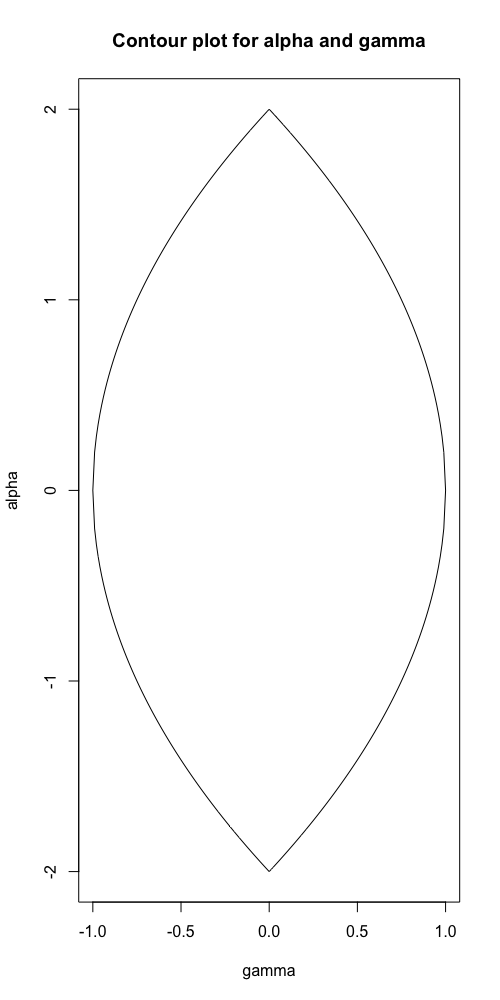
\includegraphics[scale=0.5]{Contour.png}
\centering
\caption{Geometrical interpretation of penalty function}
\end{figure}


\subsection{Criterion and Adaptive Weights} 

\subsubsection{KKT conditions}

KKT \cite{tibshirani2013lasso}

For group $\hat{\beta}^{(l)}$, the KKT condition is 

\begin{equation} \label{KKT}
  \begin{split}
  {X^{(l)}}^T(Y-X^T\hat{\beta}) &= \lambda_1\phi_l \begin{bmatrix}
         0 \\
         v 
       \end{bmatrix}
       + \lambda_1\psi_lu+\frac{1}{2}\lambda_2\hat{\beta}^{(l)}
  \end{split}
\end{equation}

where

\begin{align}
v & = \begin{cases}
  \text{sign}(\hat{\beta}_2^{(l)}) & \text{ \qquad  if $\hat{\beta_2}^{(l)}\neq 0$} \\
  \in\{v:|v|_1\leq 1\}&  \text{ \qquad  if $\hat{\beta_2}^{(l)}= 0$} 
\end{cases}
\\
u & = \begin{cases} 
  \hat{\beta}^{(l)}/\parallel \hat{\beta}^{(l)} \parallel_2 & 
  \text{ \qquad  if $\hat{\beta}^{(l)}\neq 0$} \\
  \in \{u:\parallel u\parallel_2\leq 1\} & \text{\qquad if $\hat{\beta}^{(l)}= 0$}
\end{cases} 
\end{align}

\begin{itemize}
\item We now investigate when $\hat{\beta}^{(l)}=0$ satisfies KKT condition \ref{KKT}. We propose the following condition
\begin{equation} \label{zero}
  \begin{split}
S(  {X_1^{(l)}}^T  r_{(-l)},0)^2+S(  {X_2^{(l)} }^T  r_{(-l)},\lambda_1\phi_l)^2\leq \lambda_1^2\psi_l^2
\end{split}
\end{equation}
where 

\begin{align}
S(z,a)=\text{sign}(z)(|z|-a)_+
\end{align}
and 

\begin{align}
r_{(-l)}=Y- {X^{(-l)}}^T  \hat{\beta}^{(-l)}
\end{align}

Under this condition, we can find 
\begin{align}
  u & = \begin{bmatrix}
    \frac{X_1^{(l)}r_{(-l)}}{\lambda_1\psi_l} \\
    \frac{S(  {X_2^{(l)} }^T r_{(-l)},\lambda_1\phi_l)}{\lambda_1\psi_l}
  \end{bmatrix}
  \\
  v & = \begin{bmatrix}
    0 \\
    \frac{  {X^{(l)}}^T  r_{(-l)}-S( {X_2^{(-l)}}^T r_{(-l)},\lambda_1\phi_l)}{\lambda_1\psi_l}
  \end{bmatrix}
\end{align}

such that $\parallel u\parallel_2\leq 1$ and $|v|_{\infty}\leq 1$. By simple algebra, the subgradient equation \ref{KKT}
was satisfied with $\hat{\beta}^{(l)}=0$

\item if KKT condition holds with $\hat{\beta}^{(l)}\neq 0$ but $\hat{\beta}_2^{(l)} = 0 $, the KKT condition can be reformulated as following 
\begin{align}
  {X^{(l)}}^T(Y- {X^{(-I(l))}}^T \hat{\beta}^{(-I(l))})=\lambda_1\phi_l \begin{bmatrix}
    0 \\
    v 
  \end{bmatrix}
  + \lambda_1\psi_l \frac{\hat{\beta}^{(l)}}{\parallel \hat{\beta}^{(l)} \parallel_2 } +\frac{1}{2}\lambda_2\hat{\beta}^{(l)}
\end{align}

To satisfy $\hat{\beta}_2^{(l)}=0$ and KKT condtion, we should have
\begin{align}
 {X_2^{(l)}}^T r_{(-I(l))}\leq \lambda_1\phi_l  
\end{align}
where $r_{(-I(l))}=Y- {X^{(-I(l))}}^T \hat{\beta}^{(-I(l))}$ and $I(l)$ is the interaction effect
nested in biomarker $l$th group.


\item if KKT condition holds with $\hat{\beta}^{(l)}\neq 0$ as well as $\hat{\beta}_2^{(l)}\neq 0$, the KKT condition is reformulated as

\begin{align}
  {X^{(l)}}^T(Y-  {X^{(-I(l))}}^T \hat{\beta}^{(-I(l))})=\lambda_1\phi_l \begin{bmatrix}
    0 \\
    \text{sign}(\hat{\beta}_2^{(l)})
  \end{bmatrix}
  + \lambda_1\psi_l \frac{\hat{\beta}^{(l)}}{\parallel \hat{\beta}^{(l)} \parallel_2 } +\frac{1}{2}\lambda_2\hat{\beta}^{(l)}
\end{align}

Then we get

\begin{equation} 
  \begin{split}
  \hat{\beta}_2^{(l)} & =\frac{ {X_2^{(l)}}^T (Y-X^T\hat{\beta}^{(-I(l))})-\lambda_1\phi_l\text{sign}(\hat{\beta}_2^{(l)})}{{X_2^{(l)}}^TX_2^{(l)}+\frac{\lambda_1\psi_l}{\parallel \hat{\beta}^{(l)} \parallel_2} + \frac{1}{2}\lambda_2} \\
  & = \frac{ S( {X_2^{(l)}}^Tr_{(-I(l))}, \lambda_1\phi_l ) }{ {X_2^{(l)}}^TX_2^{(l)}+\frac{\lambda_1\psi_l}{\parallel \hat{\beta}^{(l)} \parallel_2} + \frac{1}{2}\lambda_2 } 
\end{split}
\end{equation}
  
  \begin{equation} 
    \begin{split}
  \hat{\beta}_1^{(l)} & =  \frac{ {X_2^{(l)}}^T r_{(-G(l))} }{ {X_1^{(l)}}^TX_1^{(l)}+\frac{\lambda_1\psi_l}{\parallel \hat{\beta}^{(l)} \parallel_2} + \frac{1}{2}\lambda_2 } 
\end{split}
\end{equation}
  
  \begin{equation} 
    \begin{split}
  \hat{\beta}_0 & = \frac{ X_0^T r_{(-0)} }{ X_0^TX_0 } 
\end{split}
\end{equation}
  
  \begin{equation} 
    \begin{split}
  \hat{\beta}_{\tau} & = \frac{ X_T^T r_{(-T)} }{ X_T^TX_T }
\end{split}
\end{equation}

\end{itemize}

\subsubsection{Adaptive Weights}

To give each biomarker equal probability to be prognostic and predictive,
we define adaptive weights via a null model that the residual $\epsilon=r_{(-I(l))}$ 
is a normal random error where $\epsilon\sim N(0,\sigma^2)$ when $\hat{\beta}_2^{(l)}=0$.
Let
\begin{equation} \label{phil}
  \begin{split}
  \parallel {X_2^{(l)}}^T r_{(-I(l))} \parallel_2 & = \lambda_1\phi_l \\
  E[( {X_2^{(l)}}^T r_{(-I(l))})^2] & = \lambda_1^2\phi_l^2
\end{split}
\end{equation}
Thus, we can get $\lambda_1^2\phi_l^2 = \text{Var}( {X_2^{(l)}}^T r_{(-I(l))})$ and 

\begin{align}
  \phi_l & \propto \parallel X_2^{(l)} \parallel_2 
\end{align}

Since $\lambda_1$ is regularization parameter, we define $\phi_l=\parallel X_2^{(l)} \parallel_2$
without loss generality.

On the other hand, based on inequality \ref{zero} and results from formula \ref{phil}, we let
\begin{align}
  \mathbb{E} [ S( {X_1^{(l)}}^T r_{(-l)},0)^2+S( {X_2^{(l)}}^T r_{(-l)},\lambda_1\phi_l)^2  ] = \lambda_1^2\psi_l^2
\end{align}
and assume $ r_{(-l)} = \epsilon  \sim N(0,\sigma^2)$ if $\beta^{(l)}=0$, thus $\epsilon_1= {X_2^{(l)}}^T r_{(-l)} \sim N(0,\lambda_1^2\phi_l^2)$ and 
$\epsilon_0=\epsilon_1/\lambda_1\phi_l\sim N(0,1)$.



\begin{equation} \label{equ_1}
  \begin{split}
 \mathbb{E}[S( {X_2^{(l)}}^T r_{(-l)},\lambda_1\phi_l)^2] &  =  \mathbb{E}[\parallel \epsilon_1 \parallel_2^2 \mathbbm{1}_{|\epsilon_1|>\lambda_1\phi_l}]-2\lambda_1\phi_l\mathbb{E}[|\epsilon_1|\mathbbm{1}_{|\epsilon_1|>\lambda_1\phi_l}]  \\
  &  + \lambda_1^2\phi_l^2\mathbb{E}[\mathbbm{1}_{|\epsilon_1|>\lambda_1\phi_l}] \\
\end{split}
\end{equation}
  
  \begin{equation} \label{equ_2}
    \begin{split}
  \mathbb{E}[\parallel \epsilon_1 \parallel_2^2 \mathbbm{1}_{|\epsilon_1|>\lambda_1\phi_l}] & = 
  \mathbb{E}[\parallel \epsilon_1 \parallel_2^2 (1-  \mathbbm{1}_{|\epsilon_1|\leq\lambda_1\phi_l})] \\
  & = \lambda_1\phi_l^2(1- \mathbb{E}[ \parallel \epsilon_0 \parallel_2^2 ] \mathbbm{1}_{|\epsilon_0|\leq 1}  ) \\
  & \approx \lambda_1\phi_l^2(1- ( 0.68- 2 \frac{1}{\sqrt{2\pi}} \exp{(-0.5)} )  ) \\
  & = (0.32 +\sqrt{\frac{2}{\pi}}\exp(-0.5) ) \lambda_1^2\phi_l^2 \\
\end{split}
\end{equation}
  
  \begin{equation} \label{equ_3}
    \begin{split}
  \mathbb{E}[|\epsilon_1|\mathbbm{1}_{|\epsilon_1|>\lambda_1\phi_l}] & = \lambda_1\phi_l \mathbb{E}[|\epsilon_0|\mathbbm{1}_{|\epsilon_0|>1}]  \\
  & = \lambda_1\phi_l (\mathbb{E}|\epsilon_0| - \mathbb{E}|\epsilon_0| \mathbbm{1}_{|\epsilon_0|\leq 1} ) \\
  & =  \lambda_1\phi_l( \sqrt{\frac{2}{\pi}} - \sqrt{\frac{2}{\pi}} (1-\exp{(-0.5)}) )    \\ 
  & = \sqrt{\frac{2}{\pi}}\exp(-0.5) \lambda_1\phi_l \\
\end{split}
\end{equation}
  
  \begin{equation} \label{equ_4}
    \begin{split}
  \mathbb{E}[\mathbbm{1}_{|\epsilon_1|>\lambda_1\phi_l}] & = \mathbb{P}(|\epsilon_0|>1) \approx 0.32 
  \end{split}
\end{equation}

Take equations \ref{equ_2} - \ref{equ_4} to equation \ref{equ_1}, we can get

\begin{equation} \label{equ_5}
  \begin{split}
    \mathbb{E}[S( {X_2^{(l)}}^2 r_{(-l)},\lambda_1\phi_l)^2] &  \approx (0.64- \sqrt{\frac{2}{\pi}}\exp(-0.5) ) \lambda_1^2\phi_l^2
  \end{split}
\end{equation}

Insert results of equation (23) into (18), we define

\begin{equation}
  \begin{split}
\psi_l = \sqrt{\parallel X_1^{(l)} \parallel_2 + \{0.64 - \sqrt{\frac{2}{\pi}}\exp(-0.5) \} \parallel X_2^{(l)} \parallel_2} 
\end{split}
\end{equation}

such that
\begin{equation}
  \begin{split}
    \lambda_1^2\psi_l^2 = \lambda_1^2  [ \parallel X_1^{(l)} \parallel_2 + \{0.64 - \sqrt{\frac{2}{\pi}}\exp(-0.5) \} \parallel X_2^{(l)} \parallel_2 ]
  \end{split}
\end{equation}


\subsection{Algorithms}

To optimize loss function \ref{loss}, we use proximal algorithm since penalty function \ref{penalty}
is not differential everywhere \cite{liu2010fast}. Our algorithm also implements fast iterative shrinkage-thresholding algorithm with backtracking,
adaptive restart for rippling behavior, and adaptive stepwise of cyclic Barzilai-Borwein spectral approach
to accelarate convergence \cite{beck2009fast}\cite{o2015adaptive}\cite{wright2009sparse}.


Let 
\begin{equation}
Q_{\tau,g}(t,u)=\lambda_1\phi_l |t_2|_1 + \lambda_1\psi_l \parallel t \parallel_2  +\frac{1}{2\tau}\parallel t-u\parallel_2^2
\end{equation}

then the proximal operator is defined as 

\begin{equation}
\tilde{t}=arg\min_t Q_{\tau,g}(t,u)
\end{equation}

For convenience, we denote $P_{\tau,g}(u)=\tilde{t}$

To get $P_{\tau,g}(u)$, we propose the following lemma, which is generalized from fast Overlapping group lasso method \cite{liu2010fast}.

\begin{lemma}
  Define proximal operator
  \begin{equation}
    \begin{split}
    \pi_{\lambda_2}^{\lambda_1}(u) &  = arg\min_{t\in \mathbb{R}^2} \{g_{\lambda_2}^{\lambda_1 }(t) \equiv 
    \frac{1}{2\tau} \parallel t-u \parallel_2^2 + \lambda_1|t_2|_1 + \lambda_2 \parallel t \parallel_2 \} \\
    \end{split}
  \end{equation}
  The the following equition holds
  \begin{equation}
    \pi_{\lambda_2}^{\lambda_1}(u) = \pi_{\lambda_2}^{0}(v)
  \end{equation}
  where
  \begin{equation}
    \begin{split}
      v_1 & = u_1 \\
      v_2 & = \text{sign}(u_2)\max\{ |u_2|_1-\lambda_1, 0 \} \\
      \pi_{\lambda_2}^{0}(v) & = arg\min_{t\in \mathbb{R}^2} \{h_{\lambda_2}(t) \equiv 
      \frac{1}{2\tau} \parallel t-v \parallel_2^2 + \lambda_2 \parallel t \parallel_2 \} \\
    \end{split}
  \end{equation}
  \end{lemma}

  \begin{proof}
    Assume $x^* = \pi_{\lambda_2}^0(v)$ and $\phi_{\lambda_2}^{\lambda_1} (x^*) = \lambda_1|x^*_2|_1 + \lambda_2 \parallel x^* \parallel_2$. Then
    \begin{align}
      0 \in \partial h_{\lambda_2}(x^*) & = x^* -v + \partial \phi_{\lambda_2}^{0} (x^*) \\
      \partial g_{\lambda_2}^{\lambda_1}(x^*) & = x^* - u + \partial \phi_{\lambda_2}^{\lambda_1} (x^*)
    \end{align} 
    Because we have $-v+\partial \phi_{\lambda_2}^{0} (x^*) \in - u + \partial \phi_{\lambda_2}^{\lambda_1} (x^*)$, the above equations imply that $0 \in \partial g_{\lambda_2}^{\lambda_1}(x^*)$.
  \end{proof}

  Therefore, 
  \begin{equation} \label{proximal}
    \begin{split}
   P_{\tau,g}(u) &  = (1-\frac{\lambda_2}{ \parallel u \parallel_2  })_+ v  \\
   v_1 & = u_1 \\
   v_2 & = \text{sign}(u_1)\max\{|u_2|-\lambda_1\}
    \end{split}
  \end{equation}

  Based on equation \ref{proximal}, the algorithm framework is shown in Algorithm 1.


\begin{algorithm}[H]
  initialization $\theta_0=0$ or warm start from previous run, $\tau_0=0.1$, stepsize $\eta=0.5$\;
  \While{$i\le k$}{
  $u_{i}=\theta_{i-1}-\tau_i \bigtriangledown f(\theta_{i-1})$
 Find the smallest nonnegative integers $s_i$ such that with $\tau_{i}=\eta^{s_{i-1}}\tau_{i-1}$, $(f+g)(P_{\tau_i,g}(u_i))\le  Q_{\tau_i,g}(P_{\tau_i,g}(u_i),u_i)$\;
 Then, we compute $t_{i}=P_{\tau_i,g}(u_i)$
 And accelarate the computation by setting 
 \eIf{$f(\theta_{i})+g(\theta_i)>f(\theta_{i-1})+g(\theta_{i-1})$}{  $\rho_i=1$
    }{
    $\rho_i=\frac{1+\sqrt{1+4\rho_{i-1}^2}}{2}$
   }
   $\theta_i=t_i+(\frac{\rho_{i-1}-1}{\rho_i})(t_i-t_{i-1})$ and find $\tau_{i+1}$ that $\tau_{i+1}I$ can mimic the Hessian $ \bigtriangledown^2f(\theta_i)$
  }
  \caption{Patient Subgroup Identification Group Lasso Algorithm}
 \end{algorithm}
 
\subsection{Cross Validation and Regularization Parameter}

Appropriate regularization parameters, $\lambda_1$ and $\lambda_2$, are critical
for variable selection. Previous lasso methods tend to use smallest Mean Error Square(MSE)
for optimal regularization parameters. However, in this method, we will not use
MSE anymore since that will result in overfitting although the model is simplified.
So we used an arbitrary regularization parameters to select the top covariates.
But in the future, we will develop an AIC-like approach that can balance the MSE
and the model size of predictive effects. 

\section{Experiments}

We conducted several experiments to inspect how PEN will perform under
different simulation setup. Small sample size is very common in real clinical trial dataset.
That results in small $n$ and big $p$, where $n$ is sample size and $p$ is dimension. 
However, most of previous approaches used to set $n$ as
approximately 1000, which is too big to mimic a real clinical trial. 
In our experiments, we always assume
sample size is as small as 100, i.e. $n=100$. 


On the other hand, the design matrix contains 5 baseline covariates, 1 treatment
covariate and $p$ biomarkers, where $p$ is ranged from $\frac{n}{2}$ to $2n$.
Experiments with different $p$ can help us identify how the ratio $n$ and $p$
will change the variable selection. 

We also conducted different proportions of nonzero (1-sparsity) prognostic and predictive
effects from 10\% to 40\% and 5\% to 20\%, respectively. Since PEN has a strong
assumption of hierarchical structure between prognostic and predictive effects, the sparsity
of predictive biomarker is always bigger than the sparsity of prognostic biomarkers, due 
to the reason that a biomarker is prognostic before it is predictive.


To test different signal to noise ratio (SNR), PEN did variable selection on different SNR, which
is defined as $SNR=\frac{Var(X\beta)}{Var(\epsilon)}$.

Since the correlation among SNPs and biomarkers from the same pathway is common,
we also assume a blockwise AR(1) correlation structure with $\rho = .3$, where the sizes of blocks are sampling 
from multinormial distribution where the mean for block size is 5.



\begin{longtable}{|l|l|l|l|l|}
  \hline
                                                                      & Proprotion                                                       & SNR                                                          & Dimension    & SNP                                                                                                                                \\ \hline
  \endfirsthead
  %
  \endhead
  %
  \begin{tabular}[c]{@{}l@{}}\# Predictive \\ biomarkers\end{tabular} & \begin{tabular}[c]{@{}l@{}}5\%, 10\%, \\ 15\%, 20\%\end{tabular} & 10\%                                                         & 10\%         & 10\%                                                                                                                               \\ \hline
  \# Biomarkers                                                       & 100                                                              & 100                                                          & 50, 100, 200 & 100                                                                                                                                \\ \hline
  SNR                                                                 & 10                                                               & \begin{tabular}[c]{@{}l@{}}1, 5, 10, \\ 20, 100\end{tabular} & 10           & 10                                                                                                                                 \\ \hline
  Covariate Type                                                      & N(0,1)                                                           & N(0,1)                                                       & N(0,1)       & \begin{tabular}[c]{@{}l@{}}N(0,1) for baseline \\ and treatment covariates;\\ Binom(2,0.5) for genomics \\ covariates\end{tabular} \\ \hline
  \caption{Summary of Simulation Setup}
  \label{setup}\\
  \end{longtable}

  All experiments of PEN ("glasso" in tables and figures) were compared with other standard variable selection methods: 
  General Elastic Net without penalizing baseline and treatment variables (Lasso),
  Bayesian Model Averaging (BMA), Stepwise Variable Selection by likelihood (step),
  Iterative Sure Independent Screening (SIS) and Random Forest.

Table \ref{setup} shows the summary of different simulation setups we conducted.
All cases were run 100 times with fixed seed 1001-1100. The coefficients for baseline
and treatment covariates are sampled from gaussian distribution while
the coefficients for genomics covariates are constants and randomly picked up from $\pm 3$
and $\pm 5$.

\textbf{Proportion of Nonzero Predictive Effects} The proportion of nonzero
predictive effects indicates the number of biomarkers which are relate with
outcomes. Although PEN was applied on the simulation with 20\% nonzero
predictive effects, real datasets usually has much higher sparsity. Figure \ref{prop_table}
shows a comprehensive analysis with different predictive effects sparsities.
We inspected the results from several metrics: the difference between true
and estimated parameters, sum square of errors (SSE), positive predictive
value (PPV), false negative rate (FNR) and model size for only predictive 
biomarkers. Final goal for PEN is to enhance the variable selection accuracy
only for predictive biomarkers, so PPV and FNR for predictive efffects are
two mosrt important metrics.
.

From Figure \ref{prop_table} and \ref{prop_fig}, we observe that
PEN always gets almost highest PPV in all different scenerios
in the comparisons with other five methods. SIS can achieve a bit higher
PPV when proportions are 15\% and 20\%. But it is still not reliable due
to two reasons. Firstly, only proportion of $<10\%$ is practical in real
datasets. Cases of 15\% and bigger imply too much significant biomarkers.
Secondly, SIS has extremely high FNR whatever the proportion is. That is due
to the limited number of top covariates SIS selects. As shown in Figure \ref{prop_fig} (c),
the estimated predictive biomarker model size of SIS are significantly below 
the ground truth and close to axis. The other observation is that PEN
also has a slightly underestimated predictive effect model size. That is also
the key reason why PEN does not achieve the lowest FNR. That is why 
our next step is to develop a new stop criterion. Because of the arbitrary values of regularization parameters,
PEN tends to select fewer predictive biomarkers. Our future stop criterion
should guarantee an unbiased predictive biomarker model size.

\begin{figure}[t] 
  \begin{subfigure}{0.9\textwidth}
    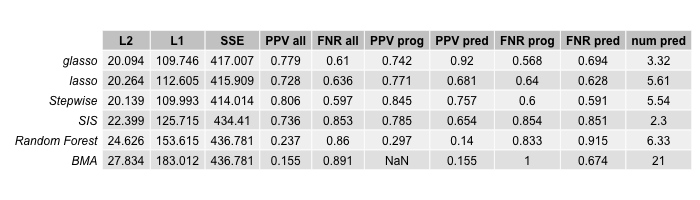
\includegraphics[width=\linewidth]{./summary/proportion/005.png}
  \caption{proportion = 5\%}
\end{subfigure}
\begin{subfigure}{0.9\textwidth}
  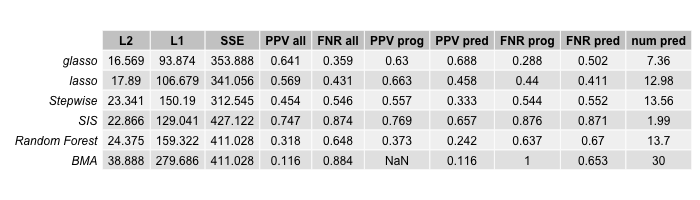
\includegraphics[width=\linewidth]{./summary/proportion/01.png}
  \caption{proportion = 10\%}
\end{subfigure}
\begin{subfigure}{0.9\textwidth}
  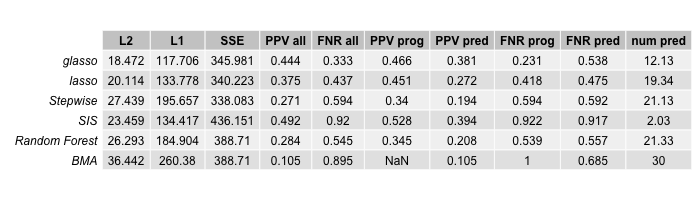
\includegraphics[width=\linewidth]{./summary/proportion/015.png}
  \caption{proportion = 15\%}
\end{subfigure}
\begin{subfigure}{0.9\textwidth}
  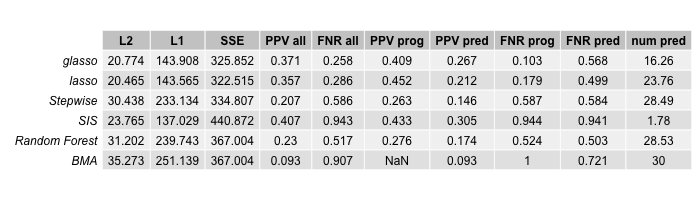
\includegraphics[width=\linewidth]{./summary/proportion/02.png}
  \caption{proportion = 20\%}
\end{subfigure}
  \centering
  \caption{Tables for different proportion when fixing the number of biomarkers as 100, 
  SNR as 10, and continuous covariate type. The proportions of nonzero predictive effects are 5\%,
   10\%, 15\%, and 20\%. L2 $=\text{mean}\parallel \hat{\beta}-\beta \parallel_2$, 
   L1 $=\text{mean}\parallel \hat{\beta}-\beta \parallel_1$, SSE = Sum Square of Errors, 
   PPV = Positive Predictive Value, FNR = False Negative Rate, num = Model Size, 
   all = across both prognostic and predictive biomarkers, prog = across only prognostic biomarkers,
   pred =  across only predictive biomarkers}
   \label{prop_table}
  \end{figure}
  
  \begin{figure}[t]
    \begin{subfigure}{0.45\textwidth}
      \includegraphics[width=\linewidth]{./summary/proportion/PPV.png}
    \caption{Precision of Predictive Biomarkers Selection}
  \end{subfigure}
  \begin{subfigure}{0.45\textwidth}
    \includegraphics[width=\linewidth]{./summary/proportion/FNR.png}
    \caption{FNR of Predictive Biomarkers Selection}
  \end{subfigure}
  \begin{subfigure}{0.45\textwidth}
    \includegraphics[width=\linewidth]{./summary/proportion/num.png}
    \caption{Model Size of Predictive Biomarkers}
  \end{subfigure}
  \begin{subfigure}{0.45\textwidth}
    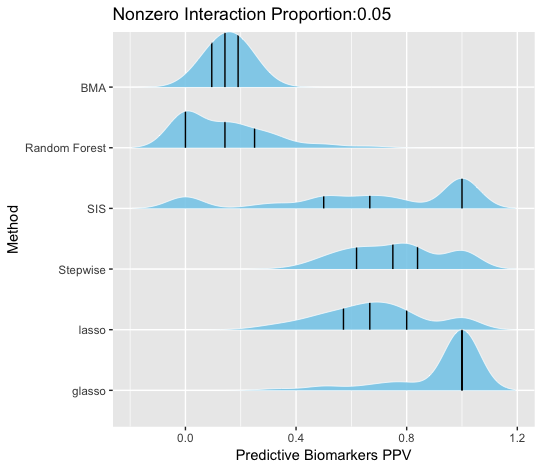
\includegraphics[width=\linewidth]{./summary/proportion/PPV005.png}
    \caption{Distribution of predictive biomarker selection precision when proportion=5\% over 100 Independent simulations.}
  \end{subfigure}
    \centering
    \caption{performance of PEN with different proportions of nonzero predictive effects.
    }
  \label{prop_fig}
\end{figure}

\textbf{SNR} Small SNR indicates large noise, e.g. half of the 
outcome variation can be explained by the noise when SNR is as small as 1.
The comprehensive data analysis and visualization of PPV, FNR and predictive
biomarker model size curves are shown in Figure \ref{SNR_table1},
\ref{SNR_table2} and \ref{SNR_fig}. Similarly, PEN always gets the best
performances in terms of PPV and FNR.

\begin{figure}[t]
  \begin{subfigure}{0.9\textwidth}
    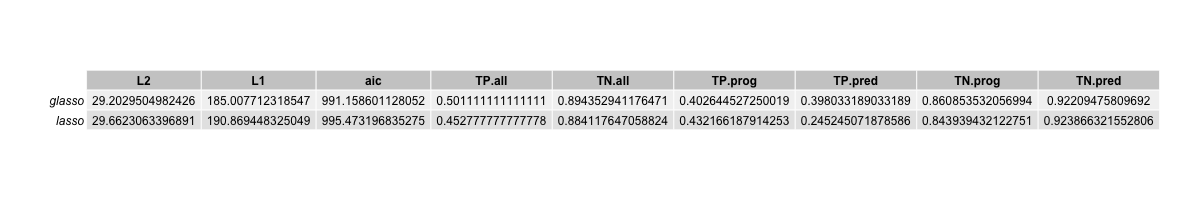
\includegraphics[width=\linewidth]{./summary/SNR/1.png}
  \caption{SNR = 1}
\end{subfigure}
\begin{subfigure}{0.9\textwidth}
  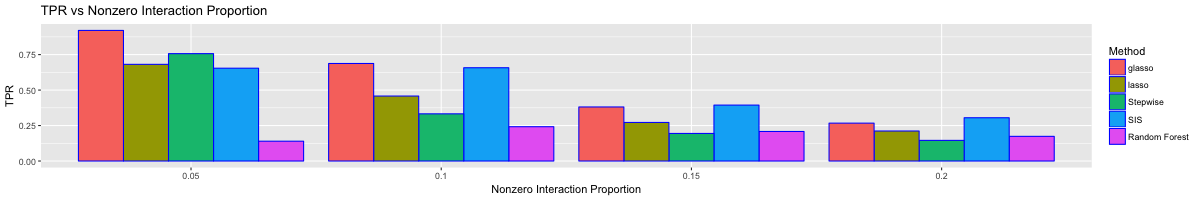
\includegraphics[width=\linewidth]{./summary/SNR/5.png}
  \caption{SNR = 5}
\end{subfigure}
\begin{subfigure}{0.9\textwidth}
  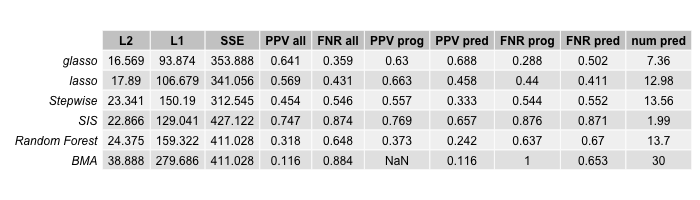
\includegraphics[width=\linewidth]{./summary/SNR/10.png}
  \caption{SNR = 10}
\end{subfigure}
 \centering
  \caption{Tables for different SNR when fixing the number of biomarkers as 100, 
  proportion as 10\%, and continuous covariate type. The proportions of nonzero predictive effects are
  1, 2, 5, and 10. }
  \label{SNR_table1}
  \end{figure}

\begin{figure}[t]
\begin{subfigure}{0.9\textwidth}
    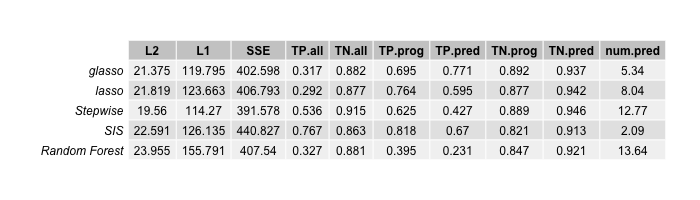
\includegraphics[width=\linewidth]{./summary/SNR/20.png}
    \caption{SNR = 20}
  \end{subfigure}
  \begin{subfigure}{0.9\textwidth}
      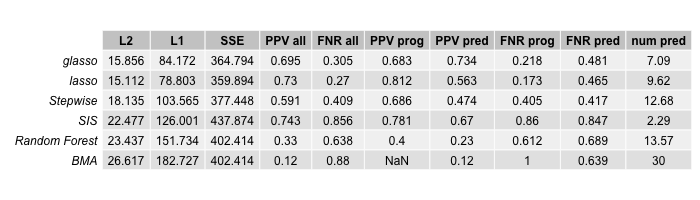
\includegraphics[width=\linewidth]{./summary/SNR/100.png}
      \caption{SNR = 100}
  \end{subfigure}
  \centering
  \caption{Tables for different SNR when fixing the number of biomarkers as 100, 
      proportion as 10\%, and continuous covariate type. The proportions of nonzero predictive effects are
      20 and 100. }
      \label{SNR_table2}
\end{figure}
  
  \begin{figure}[t]
    \begin{subfigure}{0.45\textwidth}
      \includegraphics[width=\linewidth]{./summary/SNR/PPV.png}
    \caption{Precision of Predictive Biomarkers Selection}
  \end{subfigure}
  \begin{subfigure}{0.45\textwidth}
    \includegraphics[width=\linewidth]{./summary/SNR/FNR.png}
    \caption{FNR of Predictive Biomarkers Selection}
  \end{subfigure}
  \begin{subfigure}{0.45\textwidth}
    \includegraphics[width=\linewidth]{./summary/SNR/num.png}
    \caption{Model Size of Predictive Biomarkers}
  \end{subfigure}
    \centering
    \caption{performance of PEN with different SNR.
    }
    \label{SNR_fig}
\end{figure}

\textbf{Dimension} In this session, PEN was applied on difference cases
when the number of biomarkers are 50, 100, and 200, respectively. PEN is
unable to deal with ultra high-dimensional data so far with small sample size,
i.e. $n=100$. PEN even does not have a very promising performance even with
moderate high-dimensional data, i.e. $p=2n=200$, although it is the most reliable method
compared with other methods. The problem of underestimated model size still exists for
PEN based on the results of Figure \ref{dim_fig} (c).

\begin{figure}[t]
  \begin{subfigure}{0.75\textwidth}
    \includegraphics[width=\linewidth]{./summary/n/PPV.png}
  \caption{Precision of Predictive Biomarkers Selection}
\end{subfigure}
\begin{subfigure}{0.75\textwidth}
  \includegraphics[width=\linewidth]{./summary/n/FNR.png}
  \caption{FNR of Predictive Biomarkers Selection}
\end{subfigure}
\begin{subfigure}{0.75\textwidth}
  \includegraphics[width=\linewidth]{./summary/n/num.png}
  \caption{Model Size of Predictive Biomarkers}
\end{subfigure}
  \centering
  \caption{performance of PEN with different numbers of biomarkers.
  }
  \label{dim_fig}
\end{figure}

\textbf{Categorical Covariates} For genetics data when covariates are SNPs,
binomial distribution instead of gaussian distribution can better represent the distribution of biomarkers.
Shown in Figure \ref{SNP}, PEN has an overwhelming performance in the comparisons with
the other five methods and its FNR is approximate 0.75, which is similar with the other approaches. That
indicates PEN is still the most reliable one when the covariates are SNPs.

\begin{figure}[t]
  \begin{subfigure}{0.75\textwidth}
    \includegraphics[width=\linewidth]{./summary/SNP/PPV.png}
  \caption{Precision of Predictive Biomarkers Selection}
\end{subfigure}
\begin{subfigure}{0.75\textwidth}
  \includegraphics[width=\linewidth]{./summary/SNP/FNR.png}
  \caption{FNR of Predictive Biomarkers Selection}
\end{subfigure}
  \centering
  \caption{performance of PEN with SNPs as genomics covariates.
  }
  \label{SNP}
\end{figure}


\section{Discussion}

In this project, we proposed a new method called PEN based on hierarchical group lasso
and elastic net. The special penalty term design of PEN lets it have a hierarchical 
structure between prognostic and predictive effects, which could enhance the accuracy of
predictive biomarker identification. Simulations on different scenerios have shown PEN is
a reliable approach compared with other popular methods such as Elastic Net, SIS, and random forest.
However, PEN can be further improved for a better performance. Firstly, a new stop criterion is needed for
an unbiased predictive biomarker model size. To solve this problem, it is reasonable to combine 
prediction error or likelihood with the number of selected predictive biomarkers. Secondly,
the hierarchical assumption is too strong and may not hold for some biomarkers. So we need to conduct
more experiments without such relationship. Thirdly, it is better to check whether our estimations
satisfy KKT conditions or not. That will help us to undertand the results. Finally, adaptive weights
could be improved for better estimations.


% Your references go at the end of the main text, and before the
% figures.  For this document we've used BibTeX, the .bib file
% scibib.bib, and the .bst file Science.bst.  The package scicite.sty
% was included to format the reference numbers according to *Science*
% style.


% \bibliography{scibib}

%  te\bibliographystyle{Science}

\bibliographystyle{unsrt}
\bibliography{report}



% Following is a new environment, {scilastnote}, that's defined in the
% preamble and that allows authors to add a reference at the end of the
% list that's not signaled in the text; such references are used in
% *Science* for acknowledgments of funding, help, etc.






% For your review copy (i.e., the file you initially send in for
% evaluation), you can use the {figure} environment and the
% \includegraphics command to stream your figures into the text, placing
% all figures at the end.  For the final, revised manuscript for
% acceptance and production, however, PostScript or other graphics
% should not be streamed into your compliled file.  Instead, set
% captions as simple paragraphs (with a \noindent tag), setting them
% off from the rest of the text with a \clearpage as shown  below, and
% submit figures as separate files according to the Art Department's
% instructions.


\clearpage





\end{document}




















